%
% File acl2015.tex
%
% Contact: car@ir.hit.edu.cn, gdzhou@suda.edu.cn
%%
%% Based on the style files for ACL-2014, which were, in turn,
%% Based on the style files for ACL-2013, which were, in turn,
%% Based on the style files for ACL-2012, which were, in turn,
%% based on the style files for ACL-2011, which were, in turn, 
%% based on the style files for ACL-2010, which were, in turn, 
%% based on the style files for ACL-IJCNLP-2009, which were, in turn,
%% based on the style files for EACL-2009 and IJCNLP-2008...

%% Based on the style files for EACL 2006 by 
%%e.agirre@ehu.es or Sergi.Balari@uab.es
%% and that of ACL 08 by Joakim Nivre and Noah Smith

\documentclass[11pt]{article}
\usepackage{acl2015}
\usepackage{times}
\usepackage{url}
\usepackage{latexsym}
\usepackage{graphicx}

%\setlength\titlebox{5cm}

% You can expand the titlebox if you need extra space
% to show all the authors. Please do not make the titlebox
% smaller than 5cm (the original size); we will check this
% in the camera-ready version and ask you to change it back.


\title{Sentiment Analysis within Reddit}

\author{  Matthew Nelson \\
  UC Berkeley School of Information \\
  Calgary, Alberta, CA \\
  {\tt matthewpeternelson@berkeley.edu} \\\And
  Daniel Wald \\
  UC Berkeley School of Information \\
  Los Angeles, California, USA \\
  {\tt daniel.wald@berkeley.edu} \\
  }

\date{16 December, 2017}

\begin{document}
\maketitle
\begin{abstract}
  We examine sentiment analysis within Reddit pages, calculating an overall Positivity score for an individual page as well as creating a Tree structure visualization showing the network of Positive and Negative comments within that page. We also acknowledge the difficulty of establishing accurate sentiment labels for social media literature as well as the effectiveness of a well-defined corpora in creating Sentiment Classification models. 
  
The overall accuracy of our model is \(77\%\).
  
\end{abstract}

\section{Credits}

Elements of code / models were adapted from the articles cited 
within the References section, notably ~\cite{agarwol:11} 
and ~\cite{maas:2011}. 

\section{Introduction}

The internet can be intimidating, especially for parents attempting 
to limit their children's exposure to explicit content. While the 
Children's Online Privacy Protection Act (COPA) of 1998 protects 
children under 13 from exposure to potentially explicit material 
via login credentials and privacy policy, there remains a grey area where seemingly harmless dialogue could still provide exposure to overwhelmingly negative and/or hateful content. Currently, no viable solution exists to further curtail internet access based on the dynamic scoring of text content within a webpage. To provide a solution to this problem, we build a Neural Network to extract 
an overall positivity score for individual Reddit pages, intending to predict the 
Reader's assessment of a comment's sentiment, thus providing 
a layer of information which could be utilized for additional parental controls within Reddit.

In this paper, we extract Twitter messages and train a classification model which returns one of either two
("Positive" and "Negative" in the case of the Sentiment140 Tweet Corpus Training 
Data ~\cite{agarwol:11}) or three classes ("Positive", "Negative" and "Neutral" in 
the case of the SemEval Challenge Task4a Training Data). A wealth of sentiment 
analysis work on Twitter data already exists and aspects of this contemporary 
knowledge has been leveraged in the classification sections of this report. This pre-trained model is then moved to the Reddit comment domain for practical analysis of the overall page sentiment and a visualization of each page's comment section network.

We consider three models with varied approaches to preprocessing / feature engineering. The models considered include a Multi Layer Perceptron (MLP) Neural Network, 
herein referred to as the "baseline model", Convolutional Neural Network (CNN) and 
Recurring Neural Network (RNN). All models are driven by the text contained 
within the posts themselves. In order to include the relative importance of each Reddit comment, we establish a network built on the interactions between comments, including the number of interactions and the number of chained parents 
(i.e. a 3rd order comment is in response to a 2nd order comment which is in 
turn in response to a 1st order (top level) comment or posting).

This paper is organized as follows. Section 3 outlines the methodology with 
subsections detailing the selection of corpora and models. Section 4 outlines results
of the model with subsections detailing modeling accuracy, including a discussion on human-assessed accuracy utilizing a Mechanical Turk assessment. Section 5 will discuss conclusions 
and potential improvements. Section 6 includes acknowledgements and references.

\section{Methodology}

Two separate Twitter corpora were leveraged to train a neural network model. 

Live data was then scraped from a single sub-Reddit page and fed into the model on a 
dynamic basis, creating both an overall positivity score and a visualization of the comment tree.

The model predictions were then scored for accuracy using Mechanical Turks to gather a human-assessed positive / negative score for each page. We found a \(73\%\) accuracy of the 
machine annotated corpus when measured against the human assessment and an 
individual page accuracy of \(~64\%\) when determining whether or not sub-Reddit 
pages communicated a positive or negative message overall. Possible 
errors include too small a training corpus, improper corpus categorization, 
varying degrees of decorum among Turks, and the model itself (as the models explored 
in this paper lack of complexity to discern complex communication within a comment thread such as sardonic wit, 
sarcasm or meme driven comments).

\subsection{Corpus Selection}

Two separate corpora within the social media domain were utilized in training our model, the SemEval 
Twitter Challenge Task4 corpus and the Sentiment140 corpus. Both corpora are compilations of tweets 
extracted from Twitter with categorical classifications denoting sentiment. Initially, only the 
SemEval corpus was expected to be needed in developing a model suitable for switching domains from 
Twitter to Reddit, however we found that the Accuracy on our baseline models with only the SemEval 
dataset was too low to be generalizable (more on this in section 3.1.3) and additional 
training examples were required. This motivated the use of the Sentiment140 dataset. 

\subsubsection{SemEval Twitter Challenge Task4}
The Sentiment Analysis on Twitter challenge, part of the International Workshop on Semantic Evaluation 
(SemEval), occurs once per year and asks participants to create models which can best complete a 
number of different tasks relating to the sentiment of Tweets. Task4a specifically provides a corpus 
of tweets from the previous year, human annotated with the overall sentiment of each tweet as a 
categorical Negative/Neutral/Positive and also includes the topic being discussed for each tweet. 

This challenge has been running since 2012, and download information for the training and test sets 
for each year are available on the SemEval website 
(http://alt.qcri.org/semeval2017/task4/). The SemEval challenge organizers 
have strictly obeyed Twitter's API Privacy concerns and only provided the ID of each tweet as well as 
an instructional GitHub repo explaining how to extract the tweet content from Twitter's API on your 
own. Due to the fact that some of these tweets were extracted and annotated multiple years ago, many 
attempts to pull tweets resulted in nothing being returned (tweets since deleted) and were forced out 
of our training and test sets. After combining all years of the SemEval corpus, we were able to 
utilize 16,667 valid tweets from this dataset. 

\subsubsection{Sentiment140}
The Sentiment140 corpus is a collection of 1.6 million English tweets which is available for use for 
academic purposes. The corpus consists of the 1.6 million tweets annotated with a binary 
classification of Negative / Positive. These labels were generated 
by requesting queries through the Twitter search API and specifically limiting the selection of tweets 
to those with positive and negative emoticons in their content. 
(http://help.sentiment140.com/for-students/) 

Tweets with any of [ :), :-), : ), :D, or =) ] included in the tweet were labeled as 'Positive' 
Tweets, while any tweet containing [ :(, :-(, or : ( ] were labeled as 'Negative' Tweets. 

The size of this dataset was the main justification for utilizing it, as it would 
be more effective in the generation of word/token vectors than the smaller SemEval 
dataset. However, there is some flexibility in the interpretation of why a user might 
incorporate a positive or negative emoticon in their tweet. We argue that the 
incorporation of a positive emoticon in a tweet, while not necessarily indicating that 
the tweet is itself positive, means that the author intends for the tweet to be read 
from a positive perspective. The use of a positive emoticon in 'Watching desperate 
housewives. Fun stuff.' directly explains that the user intends this to be a positive 
statement. On the contrary, the use of a negative emoticon in the above example would 
perhaps indicate a level of nuanced sarcasm that is difficult to identify without the 
help of the emoticons. In general, this makes the corpus effective in its 
interpretation of the {\em{authors intent}} behind a tweet, rather than the positive 
or negative indications from the words of the tweets themselves. 

\subsubsection{Combined Corpora}
As our initial intent was to simply understand whether a Reddit comment would be 
interpreted as positive or negative from the perspective of the person reading it we 
felt it important to allow our model to incorporate the human assessment aspect of the 
SemEval dataset (could be viewed as the Reader's perspective of Positive/Negative) 
while also benefiting from the size and variation in methodology of the Sentiment140 
dataset (could be viewed as the Writer's perspective of Positive/Negative). For this 
reason, the two corpora were concatenated together as one large dataset, with three 
categorical labels (Positive/Neutral/Negative). 

A simple chart showing the total count for Negative/Neutral/Positive (initially 
numerically mapped as 0, 2, 4) for the combined corpus is shown in Figure 
\ref{fig:Sentiment140_corpus}. Here it is evident that the count of Neutral comments 
is minuscule compared to the Positive/Negative comments (due to the fact that the 
Sentiment140 corpus was binary only and is much larger than the SemEval corpus). 

%figure at top of page 
\begin{figure}
  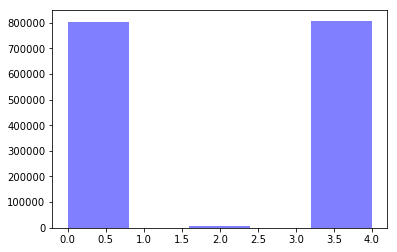
\includegraphics[width=\linewidth]{sentiment140.png}
  \caption{Sentiment140 corpus and SemEval Task4 Corpus combined, where 0 = negative, 
  2 = neutral, and 4 = positive.}
  \label{fig:Sentiment140_corpus}
\end{figure}

The decision to include the Neutral labels from the SemEval dataset was simply that the model would 
likely assign a very low probability that a tweet be labeled as Neutral and in effect it would self 
create a near-binary classification model of Positive/Negative. The inclusion of a Neutral label could easily be reversed during model training and there would be very little effect on the output predictions. 


Our baseline model was initially trailed on the following corpora: 

\begin{center}
 \begin{tabular}{||c c c||} 
 \hline
 Corpus & Entries & BL Score \\ [0.5ex] 
 \hline\hline
 SemEval 2017 & 10,000 & 52\%  \\ 
 \hline
 SemEval 2012-2017 & 16,667 & 45\%  \\
 \hline
 Sentiment140 & 1,600,000 & 76.8\%  \\
 \hline
 Cat(corpora) & 1,616,667 & 77.1\% \\[1ex] 
 \hline
\end{tabular}
\end{center}


\subsection{Baseline Model: MLP NN}

A Multi Layer Perceptron (MLP) Neural Network was used as a baseline model in an attempt to 
replicate results of some SemEval 2017 papers ~\cite{agarwol:11}. Since the end goal was to classify 
Reddit messages as either 'positive', 'negative', or neutral, we chose a multi-layer perceptron (MLP) 
neural network which specializes in categorical classification as our baseline model.

The model was trained using the SemEval 2017 corpus of ~10,000 manually 
categorized micro-blog posts. Initial execution of the model returned approximately 
52\% accuracy on test data and a one-sided prediction when applied to Twitter and 
Reddit posts. Unsure if it was simply a corpus issue, we joined our corpus with the 
last 5 years of the SemEval challenge corpora in order to grow the 
corpus into a size (~16,667 rows) that support the use of neural networks, 
yielding even worse performance. After some investigation and optimization it was 
inferred that our baseline model may have been suffering from over-fitting. At the 
same time, a parallel path was undertaken to explore the impact of the Sentiment140 
corpus on the model, motivated by the poor performance of the limited SemEval dataset 
and an understanding that neural networks perform best with hundreds of thousands to 
millions of entries. A better accuracy from the larger dataset led us to abandon the 
use of the SemEval dataset in isolation. 

\subsection{Alternative Models Explored}

Selection of the correct model relies entirely on the scope of the problem and how it 
presents in uncontrolled settings. An inspection of Reddit consumption habits reveals 
that Reddit users tend to consume comments in a more flexible manner compared to other 
domains where the Reader is forced to read sequentially. Because Reddit encourages 
users to sort based on hottest, newest or top comments, the sequential nature that most 
textual datasets form cannot be assumed within Reddit.  

As such, we chose to reject a recurring neural network 
(RNN) model because the order of consumption of comments was 
unpredictable, and because there would be contextual spill-over from parallel threads that 
cannot be accounted for in a feed forward loop. While we could accurately model a single 
comment thread, Reddit's tree structure is more complex and does not
match the ideal conditions for RNN application.

We chose to reject a convolution neural networks (CNN) for similar reasons 
as we rejected the use of RNN. This left us with an option to optimize the corpora 
as well as the MLP model.

\subsection{Tweet Feature Engineering / Preprocessing}

Multiple levels of feature engineering were used on the raw tweets in order to 
ready them for ingestion into the neural network model.

\textit{Cleaning:} Only the Sentiment and Tweet Text columns from the corpora 
were utilized, the remainder were removed including 'ItemID', 'DateTime', 'Query', 
and 'SentimentSource'.

\textit{Tokenization:} Tweets were parsed into individual tokens (words) using NLTK's TweetTokenizer function. 

\textit{Filtering:} The tokenized lists were then filtered to remove all links, 
mentions, re-tweets, handles, and emoticons [tokens that started with any of the 
strings below].
\begin{center}
 \begin{tabular}{||c c c c||} 
 \hline
 "@"  & "RT" & "\#" & "http" \\ 
 ":)"  & ":-)" & ": )" & "=)" \\ 
 ":D  & ":(" & ":-(" & ": (" \\ [1ex] 
 \hline
\end{tabular}
\end{center}


\textit{Word Vectorization:} Gensim's 
Word2Vec model (https://radimrehurek.com/gensim/) was utilized to generate a vector representation of each word, 
using 128 dimensional vectors and setting a minimum threshold on the word count 
for eligible words in order to prevent rare words (and misspellings) from 
entering the vector. 

\textit{TF-IDF Word Score:} ScikitLearn's TfidfVectorizer (http://scikit-learn.org) 
was used to generate a TF-IDF representation of the vocabulary of the corpus to 
provide a more accurate representation of each word's importance across the corpora. 

\textit{Tweet Vector:} An overall vector representation of each Word was created by
multiplying the individual Word vector by the same word's TF-IDF score. This 
multiplied word vector was then incorporated into an average Tweet vector that would 
be used as our input feature to the Neural Network Sentiment Classifier Model. This 
methodology also helps level the playing field between longer and shorter 
tweets/comments, which is very important for the transfer of the model from the Twitter 
domain to Reddit. 

\textit{Scaling:} Tweet vectors were also scaled prior to ingestion into the model. 


\subsection{MLP Optimization}

The baseline model was a simple neural network with a single layer using 
softmax activation. After investigating alternatives of CNN and RNN and deciding 
against these modeling techniques given the unique consumption style of Reddit, we 
decided to optimize the MLP baseline model.

First, we added two additional layers to assist with breaking up a purely linear model 
and modified the activation from softmax to ReLU in the first layers in order to 
optimize for a binary 
(positive/negative) output. Next, we added drop-out layers to disable a \% of neurons 
in between Dense layers in order to prevent over-fitting within the model. This yielded an 
improved accuracy for the concatenated corpora 
from 76.8\% to 77.13\%, an improvement of +0.33\%. All best practices were followed 
and only minimal improvements were observed, leading us to believe the model was 
sufficiently accurate to start obtaining results. A grid search of hyperparameters for the MLP model and feature encodings was not completed and would likely improve efficiencies slightly.

\section{Results}

Model results were largely successful in predicting whether a :) or 
:( should be attached to the sentiment (reflecting the predicted Writer's sentiment) 
mirroring the Sentiment140 corpus label structure which dominates out training set. 
Mechanical Turk analysis of 300 random sample from our corpus using a likert scale 
for Negative (1) to Positive (5) of the corpus uncovered an 18.3\% 
swing vote of tweets being labeled as Neutral, highlighting the deficiencies 
associated with a simple binary classifier system used to generate the 
sentiment140 corpus. A secondary Mechanical Turk evaluation of the corpus with a 
binary (Positive/ Negative) response showed a 73\% accuracy, similar to the results we 
extracted from the neural network model. 

\subsection{Displaying the Data}

The model is visualized using graphviz seen in Figure \ref{fig:output} to re-construct 
the parent/child relationships of comments, 
where positive messages are represented as green and negative as red. Bubble 
size represents the degree of each node within the graph structure (can also be read 
as the number of children comments stemming from that comment). The degree of each 
node was also used as a weight when generating a weighted positivity score for the 
page. An unweighted positivity score was also calculated for each page, simply taking 
into account the total number of positive and negative tweets and ignoring their 
relative importance in the graph (similarly, their likelihood to be viewed as a top 
comment). 

%figure at top of page 
\begin{figure}
  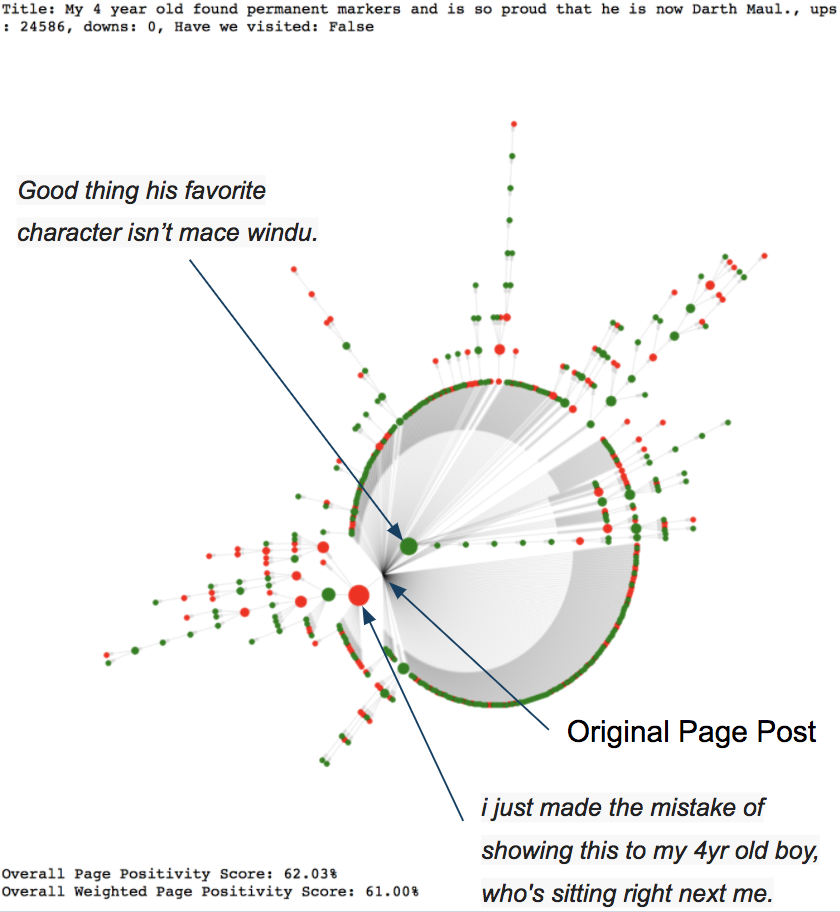
\includegraphics[width=\linewidth]{darth_maul_reddit.png}
  \caption{Annotated model output for a single Reddit page. 
  Bubble size represents number of children. Red is predicted 
  negative emoticon attached, Green is predicted positive emoticon attached. 
  \ref{fig:output}, above.}
  \label{fig:output}
\end{figure}

\subsection{Model Accuracy Discussion}

The accuracy of the final model on the combined corpus and utilizing Tweet 
Vectors as the input feature provides an accuracy of \(77.13\%\). This accuracy is 
fine, but displays the inherent challenge in using word vectors as features in order 
to predict a single classification of sentiment. However, model accuracy aside, due to 
the fact that the corpus was largely machine annotated and the conclusions we are 
making relate more to the Writer's human sentiment prediction than the Reader's, which 
was our original intent, there is some disconnect between the predicted 
classifications for Reddit comments and a human's classification. Any analysis of 
model accuracy needed to be reconciled to the levels of accuracy a human might 
provide. Thus, we employed Mechanical Turks to score 300 corpus entries as both a 
likert and binary distribution seen in figure \ref{fig:mturk_assess}, above.  

\subsubsection{Compared to Human Accuracy}

We took a snapshot of predictions and asked Mechanical Turks to complete some human 
evaluated predictions in order to obtain an unbiased 
assessment of individual posts as well as full pages / thread level positivity. Note 
there may be some jitter in these results due to the randomized differences in Turks 
as well as a self selection bias that may reflect the social 
proclivities of those that participate in the Mechanical Turk marketplace.

%figure at top of page 
\begin{figure}
  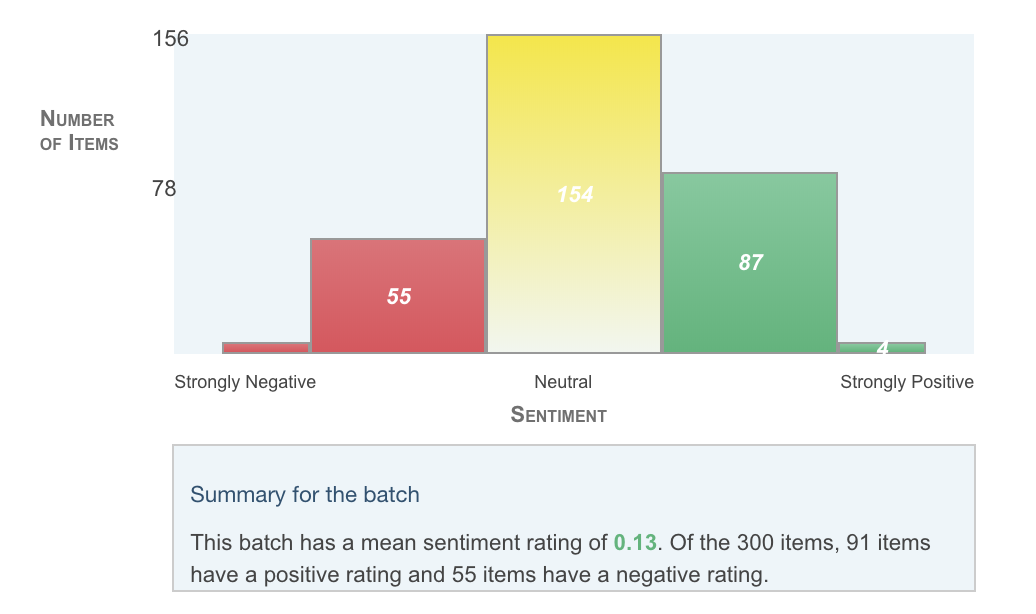
\includegraphics[width=\linewidth]{mturk_corpus_eval.png}
  \caption{Mechanical Turk evaluation of 300 sample tweets within 
  the corpus using a standard likert scale. Note the standard 
  distribution differs from corpus distribution seen in Figure 
  \ref{fig:Sentiment140_corpus}, above.}
  \label{fig:mturk_assess}
\end{figure}

Model Error was calculated by normalizing the difference 
between accuracy of the Mechanical Turk assessment and the corpus 
categorization from the model predictions, shown in the equations below:
\[
  Model = Accuracy\left(\frac{model - corpus}{model}\right)
\]
\[
  Overfit = Accuracy\left(\frac{corpus - page}{corpus}\right)
\]

Total errors are reflected in the table, below:

\begin{center}
 \begin{tabular}{||c c c||} 
 \hline
 mTurk Accuracy & Likert  & Binary  \\ [0.5ex] 
 \hline\hline
 Corpus Eval & 69\% & 73.1\% \\ 
 \hline
 Model Error & 10\% & 5\% \\
 \hline\hline
 r/portland & 59\% & -  \\
 \hline
 r/movies & - & 63.6\%  \\
 \hline
 Overfit & 14.4\% & 13\% \\[1ex] 
 \hline\hline
\end{tabular}
\end{center}

An exploration of errors shows that while a standard distribution of 
positive/negative/neutral responses is to be expected 
(Figure \ref{fig:mturk_assess}), scoring against the dominant binary 
categories in the corpus resulted in half as 
much error as with a likert analysis. Carrying these findings 
forward, we normalize the Mechanical Turk assessment of individual 
pages against the corpus accuracy to find the \% overfit remains nearly 
equivalent regardless of the scoring mechanism, providing some 
confidence that the model is performing consistently across multiple 
pages.

\section{Conclusion}

Sentiment predictions using neural networks are limited to the definitions and scope 
of the corpora used to train them. Since the model is trained based on labels 
identifying the Writer's intended
sentiment, the output provides a prediction of the Writer's sentiment sometimes conflicting 
with the Reader's sentiment.  

Our model predicted positive or negative scores (from the Writer's perspective), whereas approximately 18\% of all messages were 
interpreted by human Readers as neither positive nor negative. Our model was successful in predicting the Writer's sentiment ~77\% of the time, however when compared against a human's assessment of the same messages there remains some ambiguity. 

It is therefore the conclusion of this paper that because a Writer's intent does not always 
translate to a Reader's interpretation, the predicted labels of our Reddit classification 
system are subject to these subtle but tangible biases and the performance of our system 
did not reach the effectiveness we had desired.

\subsection{Future Improvements}

Corpus improvements can be found in two major areas. 

\textit{First,} the major source of model error was driven by the limiting corpus 
categorization and machine annotation. We assert that human annotation of the 1.6 
million tweets into at least three categorized samples would result in higher 
accuracy.  This would also change the labeling of the Sentiment140 corpus from more of 
a Writer's perspective of the tweets Sentiment to the Reader's perspective. 

\textit{Second,} the corpus distribution of positive / negative does not match the 
representation found in common Reddit pages, i.e. the swap in domains from Twitter to 
Reddit likely did not benefit the model (different forms of speech). We propose to 
randomly sample from Reddit, human annotate the comments, and create a new corpus to 
further improve and applicability of model results. 
\linebreak

Model improvements could also be extracted by considering the specific Reddit 
consumption style specified by the user. In other words, the model could be built to 
show an overall page positivity score with posts the user is more likely to encounter 
(filtered by top comments, newest comments) weighted more highly. Assuming advanced 
integration, RNN and LSTM models could also be considered by feeding one comment into 
the next to predict the overall positivity from a thread instead of individual 
comments. 

\section*{Acknowledgments}

Thank you to Ahmed Besbes' blog for baseline model inspiration 
and Dr. David Jurgens, University of Michigan School of Information, 
for model optimization consultation.

% include your own bib file like this:
%\bibliographystyle{acl}
%\bibliography{acl2015}

\begin{thebibliography}{}

\bibitem[\protect\citename{{RNN treebank}}2013]{socher:13}
{Socher, Perelygin, et al}.
\newblock 2013.
\newblock {\em Recursive Deep Models for Semantic Compositionality Over a Sentiment Treebank},
\newblock Conference on Empirical Methods in Natural Language Processing.
\newblock ~\url{http://acl2015.org/publication.html}

\bibitem[\protect\citename{{Sentiment Twitter}}2011]{agarwol:11}
{Agarwal, Xie, Vovsha, Rambow, Passonneau}.
\newblock 2011.
\newblock {\em Sentiment analysis of Twitter data}.
\newblock LSM, Portland, OR.
\newblock ~\url{https://dl.acm.org/citation.cfm?id=2021114}

\bibitem[\protect\citename{{CNN SemEval}}2017]{cliche:2017}
{Cliche}.
\newblock 2017.
\newblock {\em BB twtr at SemEval-2017 Task 4: Twitter Sentiment Analysis with CNNs and LSTMs}.
\newblock SemEval, 2017
\newblock ~\url{https://aclanthology.info/pdf/S/S17/S17-2094.pdf}

\bibitem[\protect\citename{{Sentiment Classification SemEval}}2017]{balikas:2017}
{Balikas}.
\newblock 2017.
\newblock {\em TwiSe at SemEval-2017 Task 4: Five-point Twitter Sentiment Classification and Quantification}.
\newblock SemEval, 2017
\newblock ~\url{https://aclanthology.info/pdf/S/S17/S17-2127.pdf}

\bibitem[\protect\citename{{Word Vectors for Sentiment Analysis}}2011]{maas:2011}
{Maas, Daly, Pham, Huang, Ng, Potts}.
\newblock 2011.
\newblock {\em Learning Word Vectors for Sentiment Analysis}.
\newblock Proceedings of the 49th Annual Meeting of the Association for 
Computational Linguistics, pages 142–150, Portland, OR, 2017
\newblock ~\url{http://aclweb.org/anthology/P/P11/P11-1015.pdf}

\end{thebibliography}

\end{document}